\subsection{Where Is the SLO Frontier?}
\label{sec:eval-slo}

Sweeping the soft threshold $\alpha$ from 0.55 to 0.95 at four values of $p$ moves
availability from 0.749 to 0.794 and raises the fraction of settings at which the SLO
is satisfied from 0.25 to 1.0, while the hard cap never moves: zero violations
everywhere (Fig.~\ref{fig:slo}). The knobs are not independent. At $\alpha{=}0.55$ the
monitored violation rate is 2.2\%, so the SLO holds only for $p\ge5\%$; at
$\alpha\ge0.85$ it is at most 0.22\% and the default $p{=}1\%$ holds. Operators choose
a tight target with a loose rate or the reverse, 4.5 points apart, not both: a small
set of subjects crosses any threshold near zero whatever the policy.

\begin{figure}[tb]
\centering
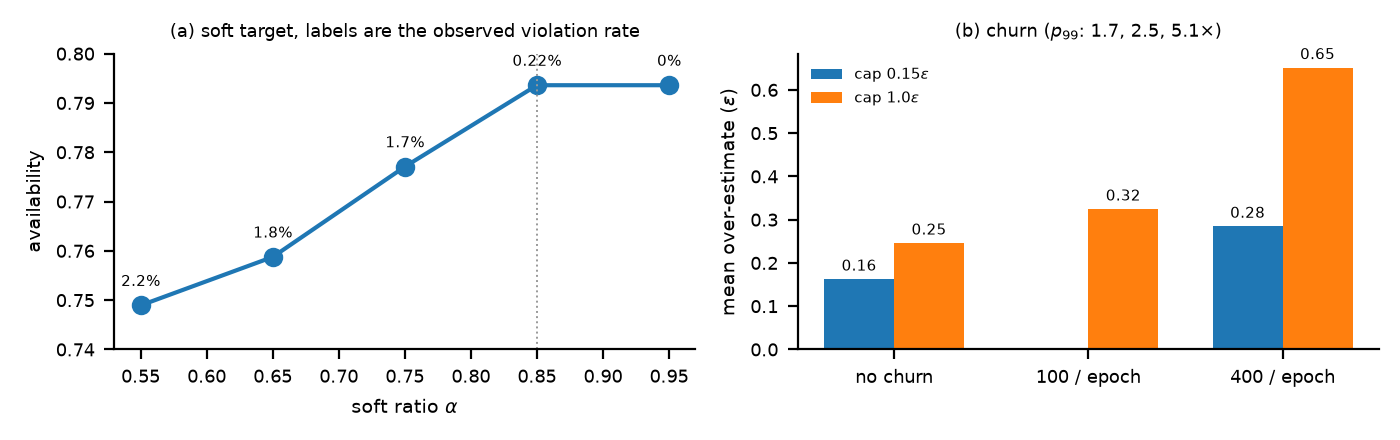
\includegraphics[width=\columnwidth]{figures/fig11_slo_churn.png}
\caption{Operating points. (a) Availability against the soft ratio, labelled with the
observed soft-violation rate; the dotted line is where the default $p{=}1\%$ starts to
hold. (b) Mean over-estimate (E14) when cohorts of heavy subjects are rotated into
the population each epoch (the $0.15\eps$ cap has no 100-cohort run); the hot table
keeps its accuracy only while churn is slow.}
\label{fig:slo}
\end{figure}

The sensitivity sweep varies one factor at a time around the default and uses a
single seed per point, so it locates trends rather than estimating their
variability. Two points bracket aggregation: with one platform, static quota becomes
sound---worst spend $0.969\eps$---because a per-tenant quota on the only platform is
also a per-subject quota; with six, its worst spend rises to $1.859\eps$ while \sys\
stays at $0.825\eps$.
A heavier tail ($\alpha_{\mathrm{zipf}}{=}1.5$) costs 15 points of availability,
from 0.936 to 0.783; 200 tenants cost 4; a 64-entry hot table costs 2; moving
$\delta$ from $10^{-6}$ to $10^{-4}$ raises availability from 0.920 to 0.941; and
crashes at 0.05 cost one point. Across all 19 points violations are zero and the
estimator never under-estimates.
